% !TEX root = allinone_main_v2.tex

\section{Cantor algebra}\label{sec:Cantor}

In this section, we recall some facts we need about Cantor algebras, and their groups of automorphisms,  the Higman--Thompson groups. We follow Higman's own account~\cite{Higman}. See also~\cite[Sec.~4]{Bro87} for a shorter survey.

%\Nnote{Higman works with~$n\ge 2$ so we need to exclude~$n=1$ early on. }

Let~$A$ be a finite set  of cardinality at least~$2$ and 
let
\[
A^*=\bigsqcup_{n\geqslant 0}A^n
\]
denote the word monoid on the set~$A$. This is the free monoid generated by~$A$, with unit~$\emptyset\in A^0$ and multiplication by juxtaposition. 
By freeness, a (right) action of the monoid~$A^*$ on a set~$S$ is uniquely determined by a map of sets~$S\times A\to S$. Such a map has an adjoint
\begin{equation}\label{eq:adjoint}
S\longrightarrow S^A=\Map(A,S).
\end{equation}

\begin{definition}\label{def:Cantor}
A {\em Cantor algebra of type~$A$} is an~$A^*$--set~$S$ such that the
adjoint structure map~\eqref{eq:adjoint} is a bijection. The morphisms of Cantor algebras of type~$A$ are the maps of~$A^*$--sets, that is the set maps that commute with the action of~$A$.  
\end{definition}
Such objects go also under the name {\em J\'onsson--Tarski algebras}.
%Ref to Smirnov? 73 or 92? or Jonsson-Tarski? probably not really necessary as it's in Wikipedia :). 

For any finite set~$X$, there exists a free Cantor algebra~$\rmC_A(X)$ of type~$A$ generated by~$X$. It can be constructed from the free~$A^*$--set 
with basis~$X$, namely the set
\[
\rmC_A^+(X):=X\x A^*=\bigsqcup_{n\geqslant 0} X\x A^n
\]
by formally adding elements so as to make the adjoint of the map defining the action bijective.~(See~\cite[Sec.~2]{Higman}; the set~$\rmC_A^+(X)$ is denoted~$X\langle A\rangle$ in \cite{Higman}.) Throughout the paper we will work with free Cantor algebras, but only the elements of the canonical free~$A^*$--set~$\rmC^+_A(X)\subset \rmC_A(X)$ will play a direct role.  



The set~$A$ will be fixed throughout the paper to be a set 
$$A=\{a_1,\dots,a_n\}$$ 
with~$n\ge 2$ ordered elements. %(Though some of our results do hold for~$n=1$, the case~$n\ge 2$ is the interesting case, so we will restrict to that. See also Remark~\ref{rem:n=1}.) 
The set~$A$ comes thus with a canonical isomorphism to the set~$[n]=\{1,\dots,n\}$, but we prefer giving it a different name to emphasize its special role. 
As for the generating set, we will be particularly interested in the case~$X=[r]=\{1,\dots,r\}$, though we will also make use of the Cantor algebras and~$A^*$--sets~$\rmC_A(E)$ and~$\rmC_A^+(E)$ generated by other sets build from~$[r]$ and~$A$. 
%in which case we will sometimes shorten the notation and just write~$\rmC_{n,r}$  for~$\rmC_{A}(X)$ and 
%$\rmC_{n,r}^+$ for~$\rmC_{A}^+(X)$. 
Note that the elements of~$\rmC_{A}^+[r]$ canonically identify with the vertices of a planar forest consisting of~$r$ rooted infinite~$n$--ary trees, as in Figure~\ref{fig:forest}. It can be useful to have this picture in mind in what follows, and interpret results using it. 
\begin{figure}[ht]
\centering
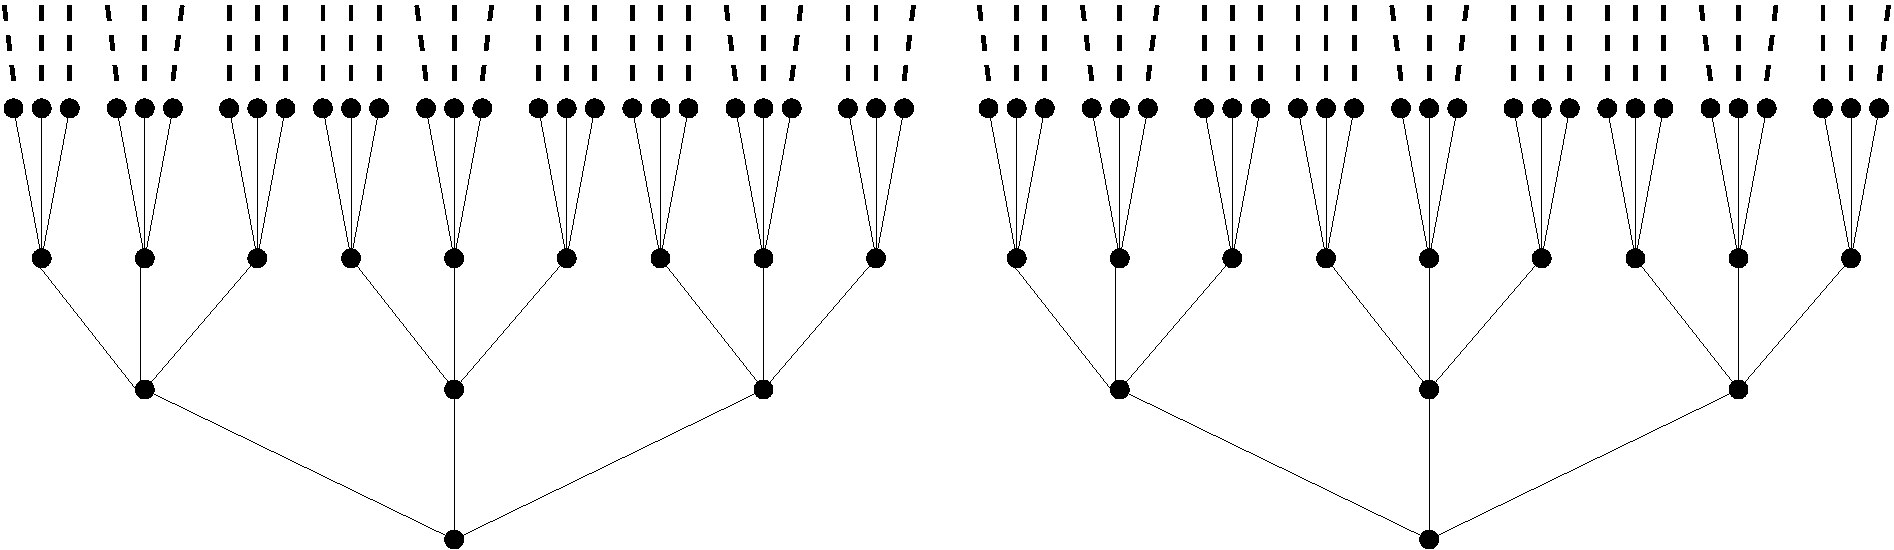
\includegraphics[width=0.7\textwidth]{forest32.pdf}
\caption{The set~$\rmC_{A}^+[2]$ for~$|A|=3$ identifies with the vertices of a forest consisting of two infinite planar ternary trees.}\label{fig:forest}
\end{figure}




Our main object of study, the Higman--Thompson groups~$\rmV_{n,r}$, are the automorphism groups of the free Cantor algebras~$\rmC_A[r]:=\rmC_{A}(X)$ for~$X=[r]$: 

\begin{definition}
Let~$A=\{a_1,\dots,a_n\}$ with~$n\geqslant 2$ and let~$r\geqslant 1$. The {\em Higman--Thompson group}
\[
\rmV_{n,r}=\Aut(\rmC_{A}[r])
\]
is the automorphism group of the free Cantor algebra of type~$A$ on~$r$ generators. 
\end{definition}

\subsection{Bases, independent sets and expansions}\label{sec:exp}

We need to understand  isomorphisms of Cantor algebras. 
By freeness, a morphism of Cantor algebras from~$\rmC_A(X)$ to a Cantor algebra~$S$ is determined by its value on the generating set~$X$.  
For instance, the canonical map~$X\x A \to \rmC_A^+(X)\to \rmC_A(X)$ induces a map~$\rmC_A(X\x A)\to \rmC_A(X)$, which one can show is an isomorphism, using the Cantor algebra structure map of~$\rmC_A(X\x A)$. An isomorphism~$f\colon\rmC_A(X)\to \rmC_A(Y)$ of Cantor algebras  can in general take the generating set~$X$ to any generating set of~$Y$. In this section, we study generating sets of Cantor algebras, in particular those called expansions, preparing for Higman's simple description of  isomorphisms between free Cantor algebras, which is recalled in the following section. 

\begin{definition}
A subset~$S\subset \rmC_A(X)$ is called 
%an {\em independent set} if the induced map~$\rmC_A(S)\to\rmC_A(X)$ is injective, and we say that~$S$ is 
a {\em  basis} for the free Cantor algebra~$\rmC_A(X)$ if  the induced homomorphism~\hbox{$\rmC_A(S)\to\rmC_A(X)$} of Cantor algebras is an isomorphism. 
%By \cite[Lem.~2.5]{Higman}, every finite independent set of~$\rmC_A^+(X)$ is contained in a finite basis also inside~$\rmC_A^+(X)$.
\end{definition} 



\begin{definition}
Given a subset~$Y$ of a free Cantor algebra~$\rmC_A(X)$, an {\em expansion} of~$Y$ is a subset of~$\rmC_A(X)$ obtained from~$Y$ by applying a {\em finite} sequence of
{\em simple expansions}, where a simple expansion replaces one element~\hbox{$y\in Y$} by the elements~\hbox{$\{y\}\x A\subset \rmC_A(X)$}, its ``descendants'' in~$\rmC_A(X)$.  For~\hbox{$Y\subset\rmC_A(X)$}, we denote by~$\calE(Y)$ the set of all expansions of~$Y$. 
\end{definition}



If~$Y$ was a basis, then so is any of its expansions \cite[Lem.~2.3]{Higman}. In particular, all the expansions of the canonical basis~$X$ represent bases for~$\rmC_A(X)$, and these are the bases we will work with. 
Note that any such basis is a finite  subset of~$\rmC_A^+(X)$. 
If we think of~$\rmC_A^+(X)$ as the vertices of an infinite~$|A|$--ary forest with roots the elements of~$X$ (as in Figure~\ref{fig:forest}), an expansion of~$X$ is the set of leaves of finite~$|A|$--ary subforest~$F$ which~``generates'' in the sense that the infinite forest is the union of~$F$ and the infinite trees attached to the leaves of~$F$. (See 
Figure~\ref{fig:basis} for an example.) %and for instance~\cite[Sec.~4]{Bro87} for more details on this point of view.)
\begin{figure}
\centering
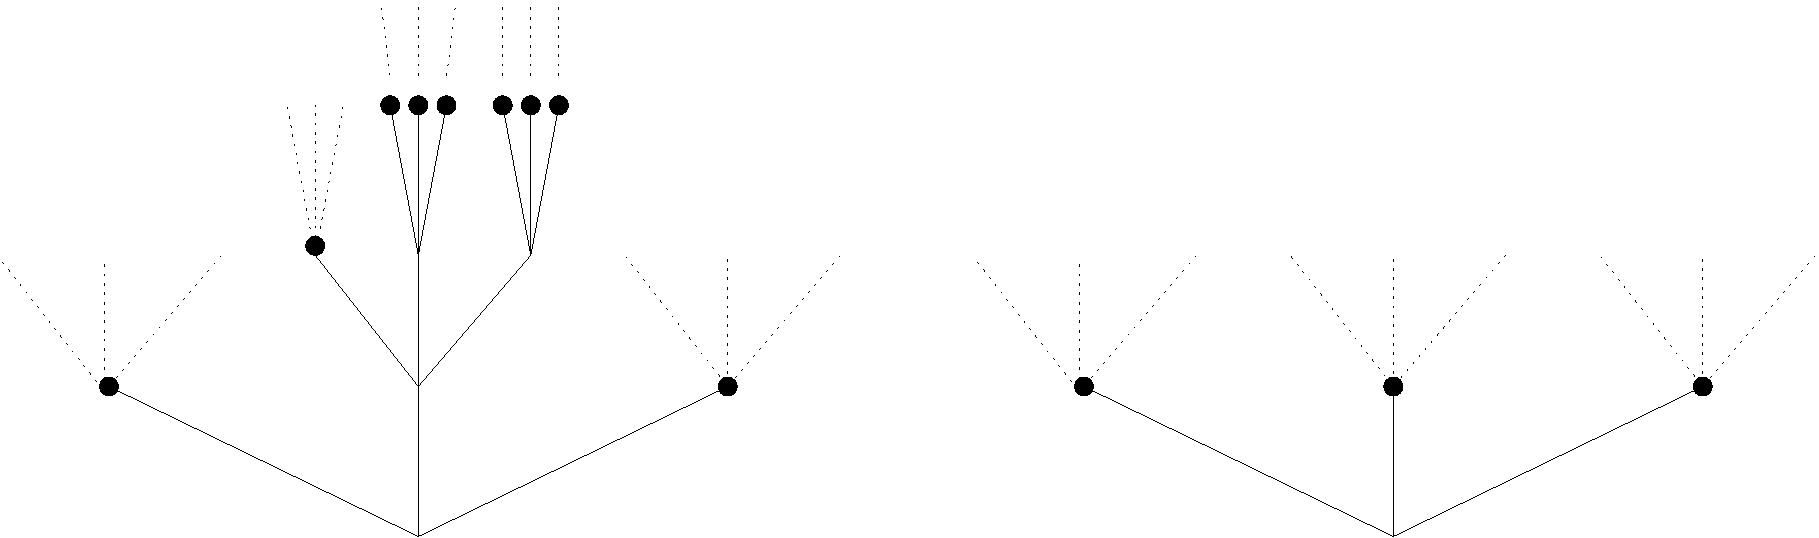
\includegraphics[width=0.7\textwidth]{basis3.pdf}
\caption{Recall the identification of~$\rmC_{A}[2]^+$ for~$|A|=3$ with the set of vertices of the forest of  Figure~\ref{fig:forest}. 
Under this identification, the vertices marked by black dots here define an expansion of the standard basis~$[2]$, obtained from it by applying a sequence of five simple expansions. This expansion has cardinality~\hbox{$12=2+5(3-1)$}.}\label{fig:basis}
\end{figure}


\begin{lem}\label{lem:expord}
The set of finite bases~$S$ of~$\rmC_A(X)$ satisfying that~$S\subset \rmC_A^+(X)$ identifies with the set~$\calE(X)$ of all expansions of~$X$. It is a partially ordered set with the relation 
$$Y\le Z \ \ \ \Longleftrightarrow\ \ \  Z \ \textrm{is an expansion of}\ \ Y.$$  
The poset~$\calE(X)$ has a least element, namely~$X$. 
\end{lem}

%Note that for~$Y,Z\in \calE(X)$, 
%$$Y\le Z \ \ \Longleftrightarrow\ \ C_A^+(Y)\supset Z \ \ \Longleftrightarrow\ \ C_A^+(Y)\supset C_A^+(Z).$$ 

\begin{proof}
We first check that the given relation~$\le$ defines a partial ordering on~$\calE(X)$: transitivity follows directly from the definition of expansion and antisymmetry follows using in addition the fact that if~$Z$ is an expansion of~$Y$, then~$|Z|\ge |Y|$, with strict inequality if the extension is non-trivial. We have that~$X\in \calE(X)$ and, by definition,~$X\le Y$ for any~$Y\in \calE(X)$, so~$X$ is a least element.  

The fact that all expansions of~$X$ are bases is given by Lemma~2.3 of \cite{Higman}, and these, by definition, lie inside~$\rmC_A^+(X)$. The fact that any finite basis that  is a subset of~$\rmC_A^+(X)$ is an expansion of~$X$ follows from Lemma~2.4 in \cite{Higman}: Suppose~$S$ is such a  basis, and let~\hbox{$U=\rmC_A^+(S)\subset\rmC_A^+(X)$}. Then~\hbox{$U=\rmC_A^+(S)\cap\rmC_A^+(X)$}, hence satisfies condition~(i) in the lemma, which is equivalent to condition~(iii) in the lemma, that is~\hbox{$U=\rmC_A^+(Z)$} for~$Z$ some expansion of~$X$. Hence~$\rmC_A^+(Z)=\rmC_A^+(S)$ as~$A^*$--subsets of~$\rmC_A^+(X)$, which is only possible if~$S=Z$ because~$S$ and~$Z$ both generate this free~$A^*$--set. 
%Then~$S\le Z$ and~$Z\le S$, and hence they must be equal. 
\end{proof}


In Section~\ref{sec:spaces} and \ref{sec:connectivity}, we will work with independent sets, which are subsets of expansions: 


\begin{definition}\label{def:independent}
A finite subset~$P\subset \rmC_A^+(X)$ is called {\em independent} if there exists an expansion~$E$ of~$X$ such that~$P\subset E$. We denote by~$\calI(X)$ the set of all independent sets of~$\rmC_A(X)$. 
If~$P,Q$ are independent sets, we will say that~$P$ is {\em independent from~$Q$} if they are disjoint and~$P\sqcup Q$ is still independent. 

We have that~$\calE(X)\subset \calI(X)$. We call the elements of~$\calI_0(X):=\calI(X)\minus \calE(X)$ the {\em non-generating independent sets}, so that the elements of~$\calI_0(X)$ are precisely the independent sets that are not bases.
\end{definition} 

When $X=[r]$, we write $\calE[r],\, \calI[r]$ and $\calI_0[r]$ for $\calE(X),\, \calI(X)$ and $\calI_0(X)$. 



\begin{lem}\label{lem:minexp}
Let~$P\in \calI(X)$ be an independent set. The subposet 
of~$\calE(X)$ of expansions of~$X$ containing~$P$ has a least element. 
\end{lem}

\begin{proof}
Suppose~$E=Q\sqcup P$ is an expansion of~$X$ containing~$P$. Consider the subalgebra of~$\rmC_A(X)$ generated by~$Q$.  
By \cite[Lem.~2.7(ii),(iii)]{Higman}, this subalgebra has a finite generating set~$G\subset \rmC_A^+(X)$ with the property that any element of its intersection with~$\rmC_A^+(X)$ is an expansion of an element of~$G$. In particular,~$Q$ is necessarily an expansion of~$G$, and~$G\sqcup P$ is the requested least element. 
\end{proof}

\begin{figure}
\centering
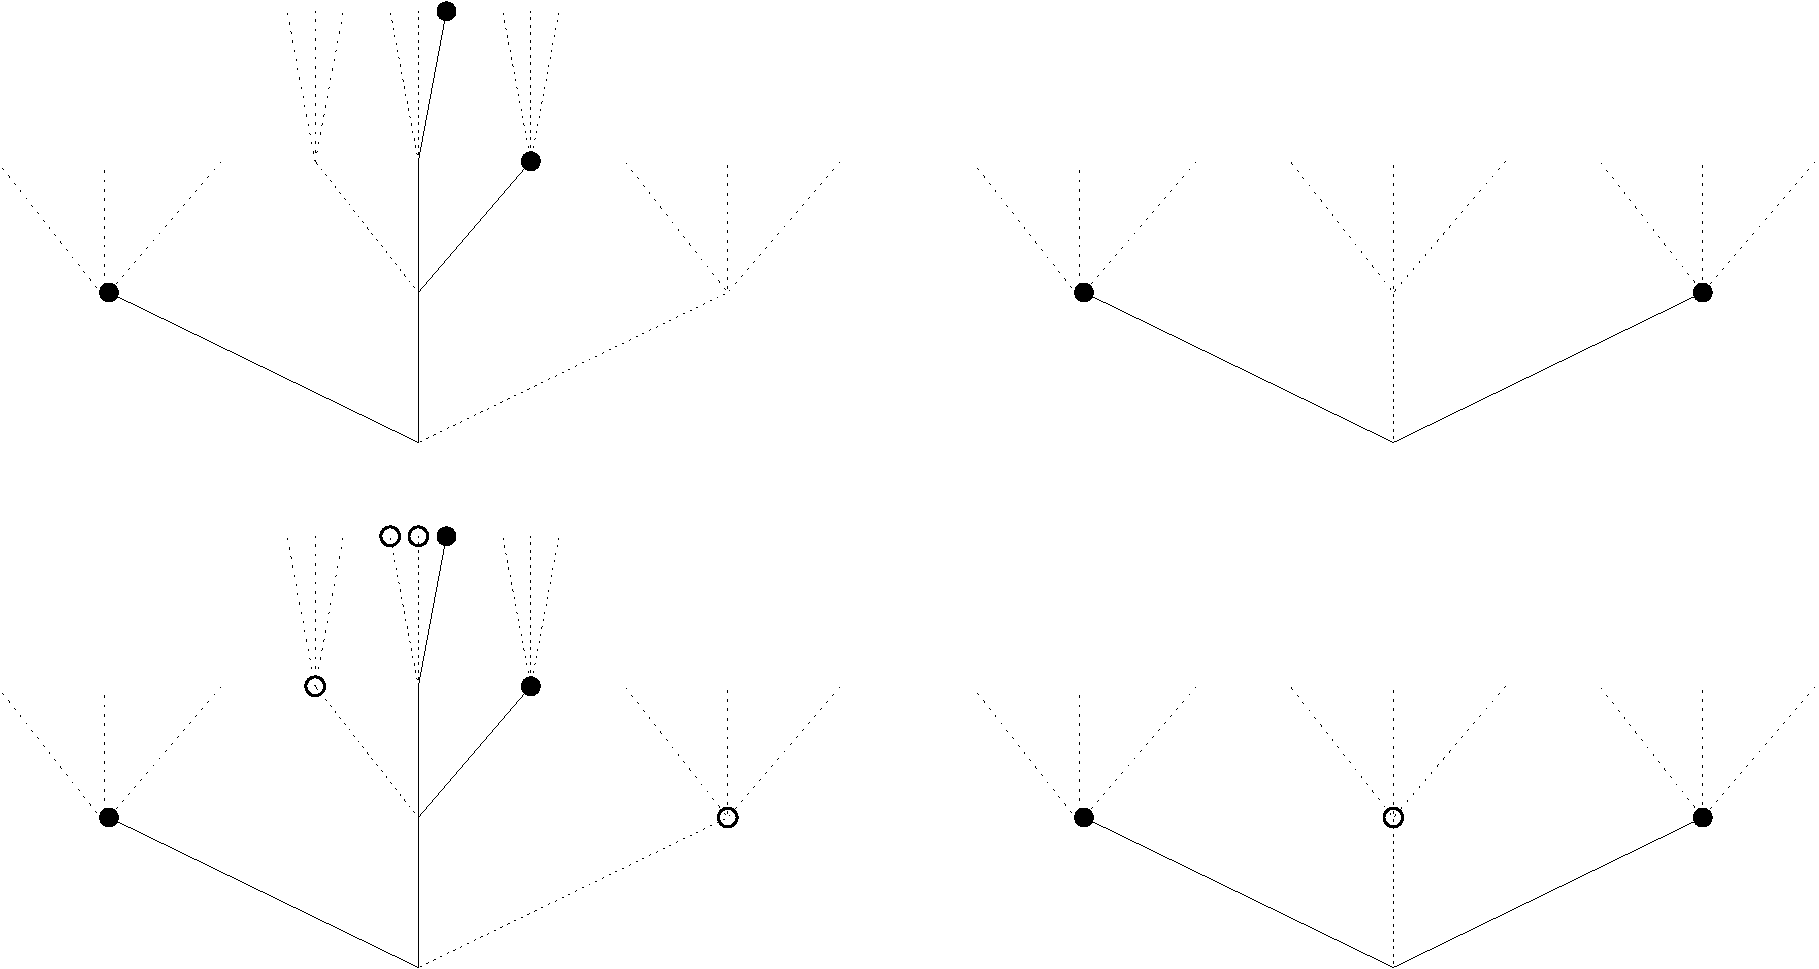
\includegraphics[width=0.7\textwidth]{indepset.pdf}
\caption{The black dots define an independent set in~$\rmC_{A}[2]^+$ for~$|A|=3$, identified with the set of vertices of the forest of  Figure~\ref{fig:forest}, and the white dots complete it to the least expansion of~$[2]$ containing it.}\label{fig:indepset}
\end{figure}




Higman proved the following important fact about bases: 

\begin{lem}{\upshape \cite[Cor.~1]{Higman}}\label{lem:common} %p12 in Higman
Any two finite bases of a free Cantor algebra have a common expansion.
\end{lem}

In particular, for any~$X$, the poset~$\calE(X)$ is directed, that is any pair of elements in~$\calE(X)$ have a common upper bound. 

A consequence of the lemma is that the cardinality of a finite basis for~$\rmC_{A}(X)$ is congruent to~$|X|$ modulo~\hbox{$|A|-1$}. In fact, for two finite sets~$X$ and~$Y$, we have that~$\rmC_{A}(X)\cong\rmC_{A}(Y)$ if and only if~\hbox{$X=\emptyset=Y$} or if~$X$ and~$Y$ are both non-empty of cardinality congruent modulo~$|A|-1$; this is the condition that guarantees that the two Cantor algebras admit finite bases of the same cardinality.




If~$X=X_1\sqcup X_2$ is the disjoint union of two finite sets, we have a canonical isomorphism
$$\rmC_A^+(X) \ \cong\ \rmC_A^+(X_1)\sqcup \rmC_A^+(X_2)$$
and more generally, the set~$\rmC_A^+(X)$ splits as a disjoint union
$$\rmC_A^+(X)=\bigsqcup_{x\in X}\rmC_A^+(\{x\}).$$
In terms of the forests of Figure~\ref{fig:forest}, we see that~$\rmC_A^+(X)$ is a disjoint union of trees, one for each element of~$X$. 
Expansions of~$X$ are subsets of~$\rmC_A^+(X)$. The following result says that the property of being an expansion can be checked componentwise.  


%Note that if~$Y$ is an expansion of~$X$, then expansions of~$Y$ are also expansions of~$X$, as~$\rmC_A^+(Y)$ is naturally a subset of~$\rmC_A^+(X)$.
\begin{lem}\label{lem:exp} Let~$S\subset \rmC_{A}^+(X\sqcup Y)$ be a finite subset. Then 
$S\in \calE(X\sqcup Y)$ if and only if~$S\cap \rmC_A^+(X)\in \calE(X)$ and~\hbox{$S\cap \rmC_{A}^+(Y)\in \calE(Y)$}, where we consider~$\rmC_A^+(X)$ and~$\rmC_A^+(Y)$ as subsets of~$\rmC_A^+(X\sqcup Y)$ through
 the identification~$\rmC_A^+(X\sqcup Y)\cong \rmC_A^+(X)\sqcup \rmC_A^+(Y)$. 
\end{lem}

\begin{proof}
Suppose first that~$S$ is an expansion of~$X\sqcup Y$, so~$S$ is obtained from~$X\sqcup Y$ by applying a finite sequence of simple expansions. Now each simple expansion is either expanding an element of~$\rmC_A^+(X)$ or of~$\rmC_A^+(Y)$, and we see that~$S=S_0\sqcup S_1$, with~$S_0$ the subset obtained by applying to~$X$ the expansions of the first type, and~$S_1$ the subset applying to~$Y$ the expansions of the second type. As~$S_0=S\cap \rmC_A^+(X)$ and~$S_1=S\cap \rmC_A^+(Y)$, this gives the first direction. The reverse direction is direct from the definition. 
%This follows from the fact that if~$E$ is an expansion of~$X$ and~$F$ an expansion of~$Y$, then~$E\cup F$ is an expansion of~$X\cup Y$, and it does not matter whether we first expand~$X$ and then~$Y$ or do it the other way around. Hence we can write any expansion of~$X\cup Y$ as the composition of an expansion of~$X$ and an expansion of~$Y$, and two such expansions are equal as expansions of~$X\cup Y$ if and only if they are equal as expansions of~$X$ and~$Y$ separately. 
\end{proof}


In fact, the lemma can be used to show that 
$$\calE(X)\cong \prod_{x\in X}\calE(\{x\})$$
as a poset. 

\subsection{Representing isomorphisms}\label{sec:isos}

Given a basis~$E$ of~$\rmC_A(X)$, a basis~$F$ of~$\rmC_A(Y)$ and a bijection~$\la\colon E\to F$, there is a unique isomorphism of Cantor algebras~$f\colon\rmC_A(X)\to \rmC_A(Y)$  that satisfies that~$f|_{E}=\la$. (Figure~\ref{fig:iso} gives an example in terms of forest.) 
But such a representing triple~$(E,F,\la)$ is far from unique. 
Indeed, any expansion~$E'$ of~$E$ defines a new such triple~$(E',F',\la')$ representing the same isomorphism~$f$ simply by taking 
$F'=f(E')$ and~$\la'=f|_{E'}$. We will now see that any isomorphism can be represented by a triple~$(E,F,\la)$ where~$E\in\calE(X)$ and~\hbox{$F\in\calE(Y)$}, and that there is in fact a canonical representative among such triples. To describe this canonical representative, we use the following partial ordering on the set of all such triples: 



\begin{figure}
\centering
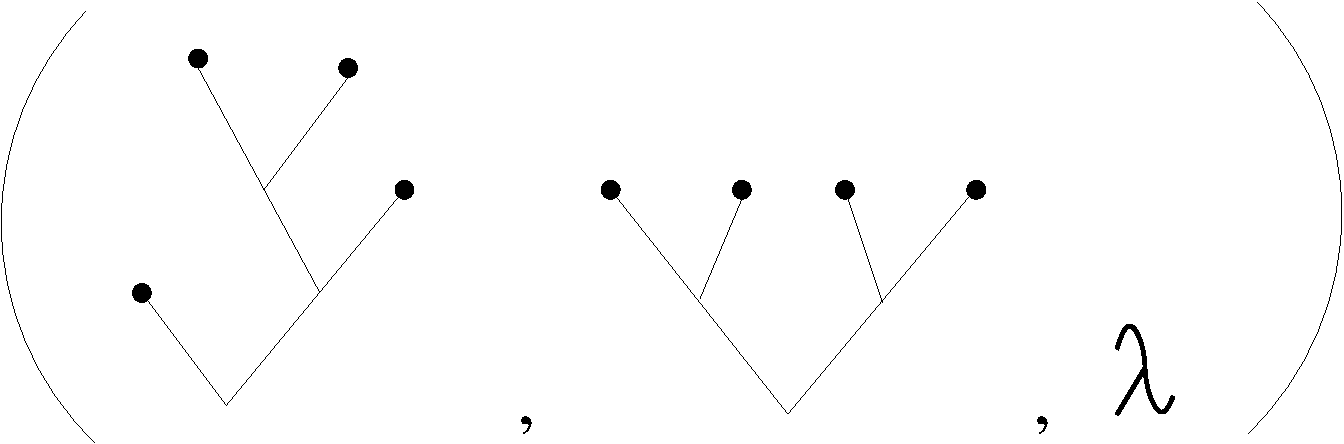
\includegraphics[width=0.4\textwidth]{iso.pdf}
\caption{Representation of an automorphism of~$\rmC_A[1]$ with~$|A|=2$ in terms of a triple~$(E,F,\la)$, where~$E$ is the set of black dots in the first tree,~$F$ the set of black dots in the second tree, and~$\la$ is some bijection between these two sets.}\label{fig:iso}
\end{figure}


\begin{Def}
For~$f\colon\rmC_A(X)\to \rmC_A(Y)$ an isomorphism of Cantor algebras, define
$$\Rep(f)=\{(E,F,\la) \ |\  E\in \calE(X), F\in \calE(Y) \ \textrm{and}\  \la=f|_E\colon E\stackrel{\cong}\rar F\}$$
to be the set of triples representing~$f$ with the property that~$E$ and~$F$ are expansions of~$X$ and~$Y$ respectively, with poset structure 
%$(E,F,\la)$,~$(E',F',\la')$ be two triple representing the same map~$f\colon\rmC_A(X)\to \rmC_A(Y)$, with~$E,E'\subset \rmC_A^+(X)$ and~$F,F'\in \rmC_A^+(Y)$. 
%We define the  
$$(E,F,\la)\le (E',F',\la') \ \  \ \Longleftrightarrow\ \ \ E\le E',$$ where the right hand side uses the partial order relation on the set~$\calE(X)$ of expansions of~$X$ 
from Lemma~\ref{lem:expord}.
\end{Def}

Note that this defines indeed a partial ordering on~$\Rep(f)$:  the transitivity follows from transitivity in the poset~$\calE(X)$, as does anti-symmetry  once one notices that~$E=E'$ forces~$F=F'$ and~$\la=\la'$ given that the triples represent the same morphism. 

Note also that having the relation~$(E,F,\la)\le (E',F',\la')$ in~$\Rep(f)$ forces the relation~$F\le F'$  in~$\calE(Y)$, because~\hbox{$F=f(E)$} and~\hbox{$F'=f(E')$}, and~$f$ takes expansions to expansions. Likewise, the map~$\la'$ under such a condition is necessarily the map induced by~$\la$ on~$E'$. 
Also, as~$F$ and~$\la$ are determined by~$E$ and~$f$, the forgetful map~$\Rep(f)\to \calE(X)$ that takes a triple~$(E,F,\la)$ to~$E$ is injective, so~$\Rep(f)$ canonically embeds as a sub-poset of~$\calE(X)$. 




The main result of the section is the following: 

\begin{prop}\label{triples}
For any isomorphism of Cantor algebras~$f\colon\rmC_A(X)\to \rmC_A(Y)$, the poset~$\Rep(f)$ is non-emtpy and has a least element. 
\end{prop}



In other words, any isomorphism~$f\colon\rmC_A(X)\to \rmC_A(Y)$ can be represented in the above sense by a triple~$(E,F,\la)$ with~$E$ an expansion of~$X$,~$F$ an expansion of~$Y$, and with~$\la\colon E\to F$ a bijection, and  there is a unique minimal such representative, with~$E$ minimal with respect to the ordering on~$\calE(X)$. 


The result is a mild generalization of~\cite[Lem.~4.1]{Higman} who gives the case~$X=Y$, and it follows from the same proof. We give it for completeness as the result is crucial for us. 

\begin{proof}
Consider the subset~$U$ of~$\rmC_A^+(X)$ defined by 
\begin{align*}U \ =\ \rmC_A^+(X)\ \cap\ f^{-1}(\rmC_A^+(Y)) %\ \cap\ \dots\cap\  f_1^{-1}\circ \dots\circ f_k^{-1}\rmC_A^+(X_k)\\
\ =\ \rmC_A^+(X)\ \cap\ \rmC_A^+(f^{-1}(Y)). %\ \cap\ \dots  \ \cap\ \rmC_A^+(f_1^{-1}\circ\dots\circ f_k^{-1}(X_k)).
\end{align*}
By \cite[Lem.~2.4]{Higman}, there exists an expansion~$E$ of~$X$ such that~$U=\rmC_A^+(E)$. As~$E$ lies inside~$U$, it satisfies that %$f_i\circ\dots\circ f_1(Y_0)$ 
$F=f(E)$ is an expansion of~$Y$. %for every~$i$. 
Taking~$(E,F,\la)$ with~$\la=f|_{E}$ yields a presentation of~$f$ with~$E$ and~$F$ expansions of~$X$ and~$Y$, which shows that~$\Rep(f)$ is non-empty. 

We also claim that the triple~$(E,F,\la)$ just constructed is in fact the least element of~$\Rep(f)$. Indeed, assume that~$E'$ is another expansion of~$X$ satisfying that~$f(E')$ 
%$f_i\circ\dots\circ f_1(Z)$
 is an expansion of~$Y$, and let~$(E',f(E'),\la')\in \Rep(f)$ be the associated triple. 
%for every~$i$. 
Then~$E'$ must lie in~$U=\rmC_A^+(E)$ and hence be an expansion of~$E$ by Lemma~\ref{lem:expord} as it is a basis of~$\rmC_A(X)$ and hence also of~$\rmC_A(E)$. 
It follows that~\hbox{$(E,F,\la)\le (E',f(E'),\la')$} in~$\Rep(f)$. 
%This proves the first part of the proposition. 
%The last statement then follows by picking~$Y_0$ to be the unique minimal expansion of~$X_0$ given by the first part of the proposition,~$Y_1$ its image by~$f$, and~$\la$ the restriction of~$f$ to~$X_0$. 
\end{proof}

\begin{ex}\label{ex:iso}
Any bijection~$\la\colon A\stackrel{\cong}\rar [n]$ induces an isomorphism~$\rmC_A[1]\stackrel{\cong}\rar \rmC_A[n]$ which is represented by the triple~$(\{1\}\x A,[n],\la)$. Its inverse~$\rmC_A[n]\to \rmC_A[1]$ is represented by the triple~$([n],\{1\}\x A,\la^{-1})$. More generally,  if $f$ is (minimally) represented by $(E,F,\la)$, then its inverse $f^{-1}$ is (minimally) represented by~$(F,E,\la^{-1})$. 
\end{ex}

\begin{rem}\label{rem:comptriples}
The composition of isomorphisms of Cantor algebras in terms of representatives can be computed as follows. If~$f\colon\rmC_A(X)\to \rmC_A(Y)$ is represented by~$(E,F,\la)$ and  
$g\colon\rmC_A(Y)\to \rmC_A(Z)$ is represented by~$(G,H,\mu)$, we have a diagram 
$$\xymatrix@R-1pc{\hat E \ar@{}[d]|\IV \ar[r]^-{\hat \la} & \hat F\ =\ \hat G \ar@{}[d]|{\IV\ \ \ \ \ \ \ \IV} \ar[r]^-{\hat \mu} & \hat H \ar@{}[d]|\IV \\
E \ar@{}[d]|\IV \ar[r]^-{\la} & F\ \ \ \ \ \  \  \  G \ar@{}[d]|{\IV\ \ \ \ \ \ \ \IV} \ar[r]^-{\mu} & H \ar@{}[d]|\IV \\
X & Y \ =\ Y  & Z
}$$
for~$\hat F=\hat G$ a common expansion of~$F$ and~$G$ (which exists by Lemma~\ref{lem:common}), and~$\hat \la$ and~$\hat \mu$ the maps induced by~$\la$ and~$\mu$, or equivalently the restrictions of~$f$ and~$g$ to~$\hat E$ and~$\hat G$, with~$\hat E:=f^{-1}(\hat F)$ and~$\hat H:=g(\hat G)$. Then the triple~$(\hat E,\hat H,\hat \mu\circ \hat \la)$ represents the composition~$g\circ f$.  Note that, even if the original representing triples were minimal, and~$\hat G$ is chosen minimally, the resulting triple representing the composition will in general not be minimal, as can be checked for instance in Example~\ref{ex:iso}. 
\end{rem}

\subsection{Categories of Cantor algebras}\label{sec:catcan}

We will in this paper work with {\em  permutative categories}, which are symmetric monoidal categories that are strictly associative and have a strict unit. By a {\em strict monoidal functor}, we will mean a monoidal functor~$F$ such that the morphisms~$F(x)\oplus F(y)\to F(x\oplus y)$ are the identity. 

Let~$\Set$ denote the category with objects the natural numbers, where we identify the integer~$r\ge 0$ with the set~\hbox{$[r]=\{1,\dots,r\}$}, and with morphisms the maps of sets. We denote by~$\Set^\x$ its subcategory of isomorphisms~(the bijections). The categories~$\Set$ and~$\Set^\x$ are both permutative categories with the monoidal structure~$\oplus$ defined using the sum on objects, and disjoint union on morphisms, using the canonical identification~$[r]\sqcup [s]\cong [r+s]$. The unit is the empty set~$[0]=\emptyset$ and the symmetry~$[r]\oplus [s]=[r+s]\to [r+s]=[s]\oplus [r]$ is given by the~$(r,s)$ block permutation. 

Let~$A=\{a_1,\dots,a_n\}$ as before. 
We now define our category~$\Can_A$ of finitely generated free Cantor algebras of type~$A$.  
To avoid set-theoretical issues, we will only consider the Cantor algebras freely generated by the sets~$[r]$ for~$r\ge 0$. So the objects of~$\Can_A$ are the natural numbers just like for the category~$\Set$, but with~$r$ now identified with the Cantor algebra~$\rmC_A[r]$. The morphisms in~$\Can_A$ are the morphisms of Cantor algebras as in Definition~\ref{def:Cantor}. We will denote by~$\Can_A^\x$ the subcategory  of isomorphisms in~$\Can_A$. 

%\begin{rem}\label{rem:n=1}
%We could have considered the case of a set~$A$ of cardinality~$1$. A Cantor algebra of type~$[1]$ is 
% \nnote{say something somewhere about the case~$A=[1]$} 
%\end{rem}

Taking the free Cantor algebra on a given set induces a  functor 
$$\rmC_A\colon\Set\rar \Can_A$$
which is the identity on objects.
Indeed, any map of sets~$[r]\to [s]$ induces a morphism~\hbox{$\rmC_A[r]\to \rmC_A[s]$} between the free Cantor algebras, because~$\rmC_A[r]$ is free on~$[r]$ and~$[s]$ canonically identifies with a subset of~$\rmC_A[s]$. This association is compatible with composition. 

\begin{Def}
For~$r<s$, we will denote by 
$$i_L\colon[r]\inc [s] \ \ \ i_R\colon[r]\inc [s]$$
the {\em left} and {\em right embeddings} of~$[r]$ into~$[s]$, i.e.~that  of~$[r]$ as the first~$r$ (resp.~last)~$r$ elements of~$[s]$. We will likewise denote by 
$$i_L,i_R\colon \rmC_A[r] \rar \rmC_A[s]$$
the corresponding induced maps~$\rmC_A(i_L)$ and~$\rmC_A(i_R)$. 
\end{Def}

We use the functor~$\rmC_A$ and the permutative structure of~$\Set$ to define a permutative structure, also denoted~$\oplus$, on 
$\Can_A$: 
On objects, we define 
\[
\rmC_A[r]\oplus \rmC_{A}[s]:=\rmC_{A}[r+s]
\]
and for morphisms~$f\colon\rmC_A[r]\to \rmC_A[r']$ and~$g\colon\rmC_A[s]\to \rmC_A[s']$, we define~$$f\oplus g\colon\rmC_A[r+s]\to \rmC_A[r'+s']$$  
to be the unique morphism defined on the basis~$[r+s]=i_L[r]\sqcup i_R[s]$ using the map 
$$[r]\ \stackrel{f|_{[r]}}\rar \ \rmC_A[r']\ \stackrel{i_L}\rar \ \rmC_A[r'+s']$$ on the first~$r$ elements and
$$[s]\ \stackrel{g|_{[s]}}\rar\  \rmC_A[s']\ \stackrel{i_R} \rar \ \rmC_A[r'+s']$$ on the last~$s$ elements. 
%where~$i_L\equiv \rmC_A(i_L)$ and~$i_R\equiv\rmC_A(i_R)$
%are the maps induced by the inclusions of sets~$i_L:[r']\inc [r'+s']$ and~$i_R:[s']\inc [r'+s']$. 
%the maps~$\rmC_A[r']\to \rmC_A[r'+s']$ and~$\rmC_A[s']\to \rmC_A[r'+s']$ are induced from the maps of sets~$[r'],[s']\to [r'+s']$. 
Finally, let 
\[
\s_{r,s}\colon\rmC_A[r+s]=\rmC_A([r]\oplus [s])\rar \rmC_A([s]\oplus [r])=\rmC_A[r+s]
\] 
be the image under the functor~$\rmC_A$ of the symmetry~$[r]\oplus [s]\to [s]\oplus [r]$ in the category~$\Set$.



\begin{prop}\label{injectiveAut}
The sum~$\oplus$ and symmetry~$\s_{r,s}$ defined above make~$\Can_A^\x$  into a  permutative category, with unit~$\rmC_A[0]=\emptyset$, with the property that 
 the free Cantor algebra functor~$\rmC_A\colon\Set^\x\to \Can_A^\x$  is a strict symmetric monoidal functor, and that the sum 
\[
\Can^\x_A(\rmC_A[r],\rmC_A[r'])\x \Can_A^\x(\rmC_A[s],\rmC_A[s'])\stackrel{\oplus}{\longrightarrow} \Can_A^\x(\rmC_A([r+s],\rmC_A[r'+s']))
\]
is injective. 
\end{prop}


One can likewise show that~$\Can_A$ is a permutative category. We restrict to~$\Can^\x_A$ for simplicity, as this is the part that is relevant to us. 

Before proving the result, we interpret the sum $\oplus$ in terms of representatives. 


We can reinterpret Lemma~\ref{lem:exp} as saying that the sum of sets~$[r]\oplus [s]=[r+s]$ extends to a sum of expansions: 
\[
\oplus\colon\calE[r]\x \calE[s]\rar \calE[r+s], 
\]
formally defined by setting~$E\oplus F=i_L(E)\sqcup i_R(F)$. (By the same lemma, this sum is an isomorphism.) Using this sum operation, we have the following: 

\begin{lem}\label{lem:sumrep}
Let~$f\in \Can_A^\x(\rmC_A[r],\rmC_A[r'])$ and~$g\in \Can_A^\x(\rmC_A[s],\rmC_A[s'])$ be isomorphisms represented by~$(E,F,\la)\in \Rep(f)$ and~$(G,H,\mu)\in \Rep(g)$. Then~\hbox{$(E\oplus G,F\oplus H,\la\oplus \mu)$} represents the sum~\hbox{$f\oplus g$}. Moreover, if~$(E,F,\la)$ is the least element of~$\Rep(f)$ and~$(G,H,\mu)$ the least element of~$\Rep(g)$, then the least element of~$ \Rep(f\oplus g)$ is~\hbox{$(E\oplus G,F\oplus H,\la\oplus \mu)$}.
\end{lem}

\begin{proof}
The sum~$f\oplus g$ is defined as the unique map taking~$i_L[r]\subset [r+s]$ to~$\rmC_A[r'+s']$ using~$i_L\circ f$ and~\hbox{$i_R[s]\subset [r+s]$} using~$i_R\circ g$. 
Now suppose that~$f$ is represented by~$(E,F,\la)$ and~$g$ by~$(G,H,\mu)$. The map of Cantor algebras~$h\colon\rmC_A[r+s]\to \rmC_A[r'+s']$ represented by~$(E\oplus G,F\oplus H,\la\oplus \mu)$ by definition takes~$i_L(E)$ to~$i_L(F)$ using~$\la=f|_{E}$ and~$i_L(G)$ to~$i_L(H)$ using~$\mu=g|_{G}$. As~$i_L(E)$ is an expansion of~$i_L[r]$ with~$i_L(F)$ the corresponding expansion of~$i_L(f[r])$, and the induced map~$h$ is a map of Cantor algebras, we necessarily have that~$h|_{i_L[r]}=i_L\circ f$, and likewise,~$h|_{i_R[s]}=i_R\circ g$. Hence~$h=f\oplus g$. 


The sum respects the poset structure by Lemma~\ref{lem:exp}. Now suppose that~$(E,F,\la)$ and~$(G,H,\mu)$ are  least elements, and that there exists~$(S,T,\nu)<(E\oplus G,F\oplus H,\la\oplus \mu)$ strictly smaller in~$ \Rep(f\oplus g)$.
By Lemma~\ref{lem:exp}, the subset~$S_0:=S\cap \rmC^+_A[r]$ is an expansion of~$[r]$. As~
$$S_0\subset \rmC^+_A[r]\subset\rmC^+_A[r+s] \ \cong \rmC_A^+[r]\sqcup \rmC_A^+[s]$$
is an expansion of~$i_L[r]$ inside~$\rmC_A[r+s]$, we have~$(f\oplus g)(S_0)=i_L\circ f(S_0)$ inside~$\rmC_A[r'+s']$, as~$f\oplus g$ restricts to~$f$ on this subset. It follows that~$(S_0,f(S_0),f|_{S_0})$ is also a representative of~$f$ which is smaller or equal to~$(E,F,\la)$. Likewise, setting~\hbox{$S_1:=S\cap \rmC^+_A[r]\subset\rmC^+_A[r+s]$}, we get a 
representative~$(S_1,g(S_1),g|_{S_1})$ of~$g$ which is smaller or equal to~$(G,H,\mu)$. Given that~\hbox{$S=S_0\oplus S_1$}, if~$S< E\oplus G$, we must have that either~$S_0<E$ or~\hbox{$S_1<G$}, contradicting the minimality assumption. Hence the sum~$\oplus$ takes least elements to least elements. 
\end{proof}

\begin{proof}[Proof of Proposition~\ref{injectiveAut}]
By the lemma, we can write the sum 
$$ \Can^\x_A(\rmC_A[r],\rmC_A[s]) \x \Can_A^\x(\rmC_A[r'],\rmC_A[s'])  \ \ \stackrel{\oplus}\rar\ \ \ \Can_A^\x(\rmC_A[r+r'],\rmC_A[s+s'])~$$
in terms of (minimal) representatives. 
Functoriality follows then from the fact that~$\rmC_A^+[r+r']\cong \rmC_A^+[r]\sqcup \rmC_A^+[r']$ and likewise for~$s,s'$, and the fact that composition can be computed componentwise. 
Associativity of the sum is likewise easily checked in this description of the sum, and~$\rmC_A[0]$ is a strict unit. For the symmetry, we need to check that 
$$\xymatrix{\rmC_A[r]\oplus \rmC_A[s] \ar[r]^-{f\oplus g} \ar[d]_{\s_{r,s}} & \rmC_A[r']\oplus \rmC_A[s'] \ar[d]_{\s_{r',s'}} \\
\rmC_A[s]\oplus \rmC_A[r] \ar[r]^-{g\oplus f} & \rmC_A[s']\oplus \rmC_A[r']   }$$
commutes for any morphism~$f,g$. In terms of representatives, one checks that if~$f$ is represented by~$(E,F,\la)$ and~$g$ by~$(G,H,\mu)$, then both compositions will be represented by 
$$(E\oplus G,H\oplus F,\widehat \s_{r',s'}\circ (\la\oplus \mu))= (E\oplus G,H\oplus F, (\mu\oplus \la)\circ \widehat \s_{r,s})$$
for~$\widehat \s_{r,s}$ the restrictions of the symmetry~$\s_{r,s}\in\Aut(\rmC_A[r+s])$ to~$E\oplus G$ and~$\widehat \s_{r',s'}$ the corresponding restriction of~$\s_{r',s'}\in\Aut(\rmC_A[r'+s'])$ to~$\la(F)\oplus \mu(G)$.  So the square commutes and 
$(\Can_A,\oplus,\s,\rmC_A[0])$ is a permutative category. 

Finally, injectivity of the sum follows, also using representatives,  from the fact that an automorphism~$f$ is uniquely represented by its least representative in~$\Rep(f)$ (Proposition~\ref{triples}), that sums of minimal representatives are minimal representatives (Lemma~\ref{lem:sumrep}),
and that the map is injective on representatives. 
\end{proof}


The following proposition will be useful in Section~\ref{sec:spaces}. 

\begin{prop}\label{prop:split}
Let~$g\colon\rmC_A[r+s]\to \rmC_A[r+s]$ be an isomorphism and suppose that~$g$ restricts to the identity on a given finite basis of~$\rmC_A[s]\equiv i_R\rmC_A[s]\subset \rmC_A[r+s]$. 
Then we have~$g=g_0\oplus \rmC_A[s]$ for some isomorphism~\hbox{$g_0\colon\rmC_A[r]\to \rmC_A[r]$}. 
\end{prop}

Here and in the following we often employ the Milnor--Moore notation and denote the identity morphism of an object by that object.

\begin{proof}
Let~$(F,G,\la)\in \Rep(g)$ be a representative of~$g$ and let~$E\subset i_R\rmC_A[s]$ be a finite basis of~$\rmC_A[s]$ fixed by~$g$. As~$F$ is an expansion of~$[r+s]$, we have that~$F_1:=F\cap i_R\rmC_A^+[s]$ is an expansion of~$[s]$ (Lemma~\ref{lem:exp}). Now~$F_1$ and~$E$ have a common expansion~$\hat E$ by Lemma~\ref{lem:common}, which is an expansion of~$[s]$ as~$F_1$ was an expansion of~$[s]$. Let~$\hat F=(F\cap i_L\rmC_A^+[r])\cup \hat E$ and~$\hat G=g(\hat F)$ and~$\hat \la=g|_{\hat F}$. 
Then~$(\hat F,\hat G,\hat \la)$ is also a representative of~$g$. Note now that~$g(\hat E)=\hat E$ and~$\hat\la|_{\hat E}=\id$ as~$g$ respects expansions and restricted to the identity on~$E$. 
%\Mnote{Is that a sentence? N: yes.}
It follows that~$\hat G=(\hat G\cap i_L\rmC_A^+[r])\cup \hat E$ for~$(\hat G\cap \rmC_A[r])$ an expansion of~$[r]$. Hence~$g=g_0\oplus \rmC_A[s]$ for~$g_0$ represented by~$(\hat F_0=F\cap i_L\rmC_A^+[r],\hat G_0=\hat G\cap i_L\rmC_A^+[r], \hat\la|_{\hat F_0})$, which proves the result.  
\end{proof}





\section{Spaces associated to Higman--Thompson groups}\label{sec:spaces}

This section and the  next one are concerned with the proof of homological stability for the Higman--Thompson groups~$\rmV_{n,r}$, the automorphism group of the free Cantor algebra~$\rmC_{A}[r]$, with respect to the number~$r$ of generators, where~$A=\{a_1,\dots,a_n\}$ as before. 
%For this part of the result, it is enough to consider the Cantor algebras~$\rmC_{n,r}$. Throughout both sections,~$n\geqslant 2$ will be fixed.  
Given a family of groups satisfying a few properties, the 
paper  \cite{Randal-Williams+Wahl}  yields  a sequence of spaces whose high connectivity implies homological stability for the family of groups. In this section, we will show how 
the groups~$\rmV_{n,r}$ fit in the framework of \cite{Randal-Williams+Wahl} and construct spaces relevant to the proof of homological stability. %, which will be given in the following section.
% as well as closely related spaces that will allow us, in the following section, to prove the necessary connectivity result. 
%Given that the variables~$n$ and~$r$ play a rather different role, we will keep on using~$$A=[n]=\{1,\dots,n\}$$ for the set with~$n$ elements. 



For a fixed type~$A$ we collect the Higman--Thompson groups into a groupoid~$\bfV_A$, which is a subgroupoid of the category~$\Can_A$, or in fact of its groupoid of isomorphisms~$\Can_A^\x$ defined in the previous section.  The objects of~$\bfV_A$ are the same as those of~$\Can_A^\x$, namely the natural numbers~$r$ as placeholders for the free Cantor algebras~$\rmC_A[r]$, and the morphism sets are defined by setting 
\begin{align*}
\bfV_A(\rmC_A[r],\rmC_A[s])=\left\{ \begin{array}{ll}  \Can^\x_A(\rmC_A[r],\rmC_A[s]) & r=s\\
\emptyset & r\neq s
\end{array}\right.
\end{align*}
In other words,~$$\bfV_A\cong \bigsqcup_{r\ge 0}\rmV_{n,r}$$ is the groupoid of {\em automorphisms} in~$\Can_A^\x$, with each group~$\rmV_{n,r}$ considered as a groupoid with one object. Recall that there are isomorphisms~$\rmC_{A}[r]\cong\rmC_A[r+(n-1)]$ for any~$r\geqslant1$ (with~$n=|A|$). These isomorphisms are morphisms in the groupoid~$\Can^\x_A$  but we do {\em not} include these isomorphisms into the groupoid~$\bfV_A$. 
Note that the symmetric monoidal structure of~$\Can_A^\x$ restricts to~$\bfV_A$, making it a permutative groupoid. 

\subsection{Homogeneous categories}\label{sec:homogeneous}



Recall from~\cite[Def.~1.3]{Randal-Williams+Wahl} that a monoidal category~$(\bfH,\oplus,0)$ is called {\em homogeneous} if the monoidal unit~$0$ is initial and if the following two conditions are satisfied for every pair of objects~$X, Y$ in~$\bfH$: The set~${\bfH}(X,Y)$ is a transitive~$\Aut_{\bfH}(Y)$--set under post-composition, and the homomorphism
\[
\Aut_{\bfH}(X)\to\Aut_{\bfH}(X\oplus Y)
\]
that takes~$f$ to~$f\oplus Y$ is injective with image~$\{\phi\in\Aut_{\bfH}(X\oplus Y)\ |\phi\circ (\iota_X\oplus Y)=\iota_X\oplus Y\}$. %, the stabilizer of the image of~$\iota_A$.
The main examples of homogeneous categories can be obtained by applying Quillen's bracket construction to a groupoid. We recall this construction here, and show that it yields a homogeneous category when applied to the groupoid~$\bfV_A$. 

Let~\hbox{$\bfQ_A=\langle\bfV_A,\bfV_A\rangle$} denote the category obtained by applying Quillen's bracket construction~(see~\cite[p.~219]{Grayson:QuillenII}) to the groupoid~$\bfV_A$.  The category~$\bfQ_A$ has the same objects as~$\bfV_A$ and there are no morphisms from~$\rmC_A[r]$ to~$\rmC_A[s]$ unless there exists a~$k$ such that~\hbox{$\rmC_A[k]\oplus\rmC_A[r]\cong\rmC_A[s]$} in~$\bfV_A$, i.e.~$r\leqslant s$ in our case, with~\hbox{$k=s-r$}. If this is the case, morphisms are equivalence classes~$[f]$ of morphisms~$f$ in~$\rmV_{n,s}=\Aut_{\bfV_A}(\rmC_A[s])$ with~$f\sim f'$ if there exists an element~$g$ in~$\rmV_{n,k}$ such 
that
\[
f'=f\circ (g\oplus\rmC_A[r])\colon\ \rmC_A[s]=\rmC_A[k]\oplus\rmC_A[r]\ \rar\ \rmC_A[s].
\] 
Note that the unit~$\emptyset=\rmC_A[0]$ is now an initial object in the category~$\bfQ_A$. We will write~\hbox{$\iota_{r}\colon\emptyset\to\rmC_A[r]$} for the unique morphism, which we can represent as the equivalence class~$[\rmC_A[r]]$ of the identity in~$\rmV_{n,r}$. 


\begin{proposition}
The category~$\bfQ_A$ is a permutative and homogeneous category with maximal subgroupoid~$\bfV_A$.   
\end{proposition}

\begin{proof} This is a direct application of three results in~\cite{Randal-Williams+Wahl}: Because~$(\bfV_A,\oplus,\s,\emptyset)$ is a symmetric monoidal groupoid,~\cite[Prop.~1.7]{Randal-Williams+Wahl} gives that~$\bfQ_A$ (denoted~$U\bfV_A$ in that paper) inherits a symmetric monoidal structure, with its unit~$\emptyset$ initial. And given that~$\bfV_A$ was actually permutative, so is~$\bfQ_A$. 
We have that~$\Aut(\emptyset)=\{\id\}$ and that there are no zero divisors in~$\bfQ_A$: If there is an isomorphism~$\rmC_A[r]\oplus\rmC_A[s]\cong\emptyset$ in~$\bfV_A$, then we must have that~$r=s=0$. Then~\cite[Prop.~1.6]{Randal-Williams+Wahl} gives that~$\bfV_A$ is the maximal subgroupoid of~$\bfQ_A$. Also, the groupoid~$\bfV_A$ satisfies cancellation~(by construction): If there exists an isomorphism~$\rmC_A[r]\oplus\rmC_A[s]\cong\rmC_A[r]\oplus\rmC_A[s']$ in~$\bfV_A$, then~\hbox{$\rmC_A[s]\cong\rmC_A[s']$} in~$\bfV_A$; they are in fact equal, because we have~\hbox{$\rmC_A[r+s]\cong\rmC_A[r+s']$} in the groupoid~$\bfV_A$ if and only if~$r+s=r+s'$. Finally, the groupoid~$\bfV_A$ satisfies that the map~\hbox{$\Aut_{\bfV_A}(\rmC_A[r])\to\Aut_{\bfV_A}(\rmC_A[r+s])$} adding the identity on~$\rmC_A[s]$ is injective by Proposition~\ref{injectiveAut}. It then follows from~\cite[Thm.~1.9]{Randal-Williams+Wahl} that~$\bfQ_A$ is homogenous, which completes the proof. 
\end{proof}

%\begin{remark}
%In fact, we have forced cancellation in the groupoid~$\bfV_a$ by forgetting the isomorphisms displayed in Example~\ref{isoex}. Including all isomorphisms of Cantor algebras in the groupoid, we would have had that~$\rmC_1\oplus\rmC_{n-1}=\rmC_a\cong\rmC_1=\rmC_1\oplus\rmC_0$, giving a counter-example to cancellation, because~$\rmC_{n-1}$ is not isomorphic to~$\rmC_0$.
%\end{remark}



\begin{remark}\label{rem:comp}
Explicitly, the monoidal structure of~$\bfQ_A$ is defined as follows. On objects, it is as in~$\bfV_A$ induced by the sum of natural numbers. Given two morphisms~$[f]\in \bfQ_A(\rmC_A[r],\rmC_A[s])$ and~\hbox{$[g]\in \bfQ_A(\rmC_A[r'],\rmC_A[s'])$}, the equivalence class of the composition
\[
\xymatrix{\rmC_A[s+s']\ar@{=}[r]&\rmC_A[s-r]\oplus\rmC_A[s-r']\oplus\rmC_A[r]\oplus\rmC_A[r']\ar[d]^{\rmC_A[s-r]\oplus\sigma_{s-r',r}\oplus\rmC_A[r']} & &\\ 
&\rmC_A[s-r]\oplus\rmC_A[r]\oplus\rmC_A[s-r']\oplus\rmC_A[r']\ar@{=}[r]&\rmC_A[s]\oplus\rmC_A[s']\ar[d]^-{f\oplus g}\\
 &&\rmC_A[s]\oplus\rmC_A[s']\ar@{=}[r]&\rmC_A[s+s'].}
\]
defines~$[f]\oplus [g]\in \bfQ_A(\rmC_A[r+r'],\rmC_A[s+s'])$, where~$\sigma_{s-r',r}$ is the symmetry of~$\bfV_A$. (See the proof of Proposition~1.6 in \cite{Randal-Williams+Wahl}.) 
\end{remark} 

%%%

\subsection{Representing morphisms in the category~$\bfQ_A$}



Recall from Proposition~\ref{triples} that the isomorphisms of~$\Can_A$, and hence also the elements~$f$ of~$\rmV_{n,s}$, admit a unique minimal
presentation~$(E,F,\la)$ where~$E,F$ are expansions of the standard generating set~$[s]$
of~$\rmC_A[s]$, and~$\la\colon E\to F$ is a bijection. 
We will now define an analogous minimal representation for the morphisms in~$\bfQ_A(\rmC_A[r],\rmC_A[s])$ for~\hbox{$r<s$}.
This description makes use of the posets~$\calE[r], \, \calI[r]$ and $\calI_0[r]$ of  expansions, independent sets, and non-generating independent sets of~$[r]$ of Section~\ref{sec:exp}. 




An element~$[f]\in \bfQ_A(\rmC_A[r],\rmC_A[s])$ is represented by some~$f\in \rmV_{n,s}$, which itself admits a representative~$(E,F,\la)$, with~$E,F\in \calE[s]$ expansions of~$[s]$ and~$\la\colon E\to F$ a bijection. Using the decomposition 
$$[s]=[s-r]\oplus [r],$$ 
with the associated embedding~$i_R\colon\rmC_A^+[r]\inc \rmC_A^+[s]$, 
we can consider the intersection~$E_0:=E\cap i_R\rmC_A^+[r]$, which is an expansion of~$[r]$ by Lemma~\ref{lem:exp}. Then~\hbox{$P:=\la(E_0)\subset \la(E)=F$} is an independent set of~$\rmC_A[s]$. This way we can associate to any morphism~$[f]\in \bfQ_A$ a triple~$(E_0,P,\la)$ with~$E_0\in \calE[r]$ and~$P\in \calI[s]$ and~$\la\colon E_0\to P$ a bijection. 
With this in mind, we extend the definition of~$\Rep(f)$ from Section~\ref{sec:isos} to all morphisms of~$\bfQ_A$: 
\begin{Def}
For~$[f]\in \bfQ_A(\rmC_A[r],\rmC_A[s])$, let 
$$\Rep[f]=\{(E,P,\la)\ |\ E\in \calE[r], P\in \calI[s], \la=[f]|_E\colon E\stackrel{\cong}\rar P\},$$
which we consider as a poset by setting~$(E,P,\la)\le (E',P',\la')$ if and only if~$E\le E'$ in~$\calE[r]$.  
\end{Def}

Note that~$[f]|_E$ is a well-defined map as~$E\subset \rmC_A[r]\equiv i_R\rmC_A[r]$ and any two representatives of~$[f]$ agree as maps on that subalgebra. 

If~$r=s$, we have that~$\Rep[f]=\Rep(f)$ as defined earlier. In particular, if~$(E,P,\la)\in \Rep[f]$ in this case, then~$P\in \calE[s]$. On the other hand, if~$r<s$ and~$(E,P,\la)\in \Rep[f]$, we must have that~$P\in \calI_0[s]$ as~$P$ is non-generating in that case. 
Proposition~\ref{triples} extends to the following result: 

\begin{prop}\label{triples2}
For any morphism~$[f]\in \bfQ_A(\rmC_A[r],\rmC_A[s])$, the set~$\Rep[f]$ is non-empty and has a least element. 
\end{prop}


\begin{proof}
We have already seen above that the set is non-empty. We will in this proof construct a least element. Pick a representative~$f\in \rmV_{n,s}$ of~$[f]$, and let~$(E,F,\la)$ be the least element of~$\Rep(f)$ given by Proposition~\ref{triples}. As above, we consider the set~$[s]$ as the sum~$[s-r]\oplus [r]$, which gives embeddings~$i_L$ and~$i_R$  of~$\rmC_A[s-r]$ and~$\rmC_A[r]$ inside~$\rmC_A[s]$. 
Consider the triple~$(E_0,P,\la|_{E_0})$ with~$E_0=E\cap i_R\rmC_A^+[r]$ and~$P=\la(E_0)$. We have that~$E_0\in \calE[r]$ by Lemma~\ref{lem:exp} and~$P\in \calI[s]$ because~$P\subset \la(E)=F$. Given that~$f|_E=\la$, we get that 
$(E_0,P,\la|_{E_0})\in \Rep[f]$. We claim that~$(E_0,P,\la|_{E_0})$ is the least element of~$\Rep[f]$. So suppose~$(E_0',P',\la')\in \Rep[f]$ is another element. Set~$$E'=(E\cap i_L\rmC_A^+[s-r])\cup E_0'.$$ By Lemma~\ref{lem:exp}, we have~$E'\in \calE[s]$, and hence this is a basis for~$\rmC_A[s]$. 
%Suppose that~$E'_0\le E_0$. Then we also have~$E'\le E$. Note also that 
Now~$f(E')=f(E\cap \rmC_A^+[s-r])\cup P'$ is a basis, as~$f$ is an isomorphism, and it is included in~$\rmC_A^+[s]$ as both~$f(E\cap \rmC_A^+[s-r])$  and~$P'$ are. Hence it is an expansion of~$[s]$ by Lemma~\ref {lem:expord} and~$(E',f(E'),f|_{E'})$ is an element of~$\Rep(f)$. By the minimality of~$(E,F,\la)$, we must have that~$E\le E'$, which gives~$E_0\le E_0'$ as requested. 
\end{proof}


Define 
$$\rmP_A(r,s)=\left\{ \begin{array}{ll} \{(E,P,\la)\ |\ E\in\calE[r], P\in\calI_0[s], \la\colon E\stackrel{\cong}\rar P\}  & \textrm{if}\ \ r<s\\
\{(E,P,\la)\ |\ E\in\calE[r], P\in\calE[s], \la\colon E\stackrel{\cong}\rar P\}  & \textrm{if}\ \ r=s. \end{array}\right.$$
%\end{itemize} 
%\begin{itemize}
%\item~$E\subset \rmC_{n,r}^+$ is an expansion of the canonical basis~$[r]$, 
%\item~$P\subset \rmC_{n,s}^+$ is an independent set which is not a basis, %which is a basis if and only if~$r=s$,  
%\item~$\la\colon E\to P$ is bijection
%\end{itemize} 
We partially order~$\rmP_A(r,s)$ by setting~\hbox{$(E,P,\la)\leqslant (E',P',\la')$} if and only if~$E\le E'$ and~$\la'$ is the restriction to~$E'$ of the map~$\rmC_A(E)\to \rmC_A(P)\to \rmC_A[s]$ induced by~$\la$. As~$P'=\la'(E')$, it follows that~$P'$ is an expansion of~$P$ in such a situation.
%with~$A=[n]$ as above. 

\begin{prop}\label{prop:morphisms}
For all~$0\leqslant r\leqslant s$, there is a poset isomorphism~$$\rmP_A(r,s)\cong \bigsqcup_{[f]\in \bfQ_A(\rmC_A[r],\rmC_A[s])}\Rep[f].$$
In particular, taking least representative in~$\Rep[-]$ defines an isomorphism between~$\bfQ_A(\rmC_A[r],\rmC_A[s])$ and the set of minimal elements in~$\rmP_A(r,s)$. 
%A morphism~$[f]\colon\rmC_r\to\rmC_s$ in~$\bfQ_a$ with~$r\leqslant s$ is determined by a triple~$(F=F_1\sqcup\dots\sqcup F_r,G=G_1\sqcup\dots\sqcup G_s;\lambda)$ for~$F$ an~$(n,r)$--forest,~$G$ an~$(n,s)$--forest, and~$\lambda\colon L(F)\to L(G)$ an injective map which is surjective if and only if~$r=s$. Moreover, every such triple represents a morphism in~$\bfQ_a$, and for each morphism of~$\bfQ_a$, there is a unique minimal representative under expansion. 
%
%Alternatively, we can represent a morphism from~$\rmC_r$ to~$\rmC_s$ as a pair~$(B,\la)$ where~$B$ is a basis for~$\rmC_{n,r}$ and~$\la\colon B\to\rmC_{a,s}$ is an injective map with image an {\color{red}independent} set, which is a basis if and only if~$r=s$.  
\end{prop}




\begin{proof}
Forgetting which~$[f]$ a triple represents defines  a  map 
$$\al\colon\bigsqcup_{[f]\in \bfQ_A(\rmC_A[r],\rmC_A[s])}\Rep[f] \ \rar\ \rmP_A(r,s)$$
which is a map of posets as the order relation is defined in the same way in both cases. We want to show that this map is a poset bijection, that is a set bijection such that any two elements that are related in the target, are also related in the source, or equivalently, that any two elements that are related  in~$\rmP_A(r,s)$ represent the same morphism~$[f]$. 

When~$r=s$,  any element~$(E,P,\la)\in \rmP_A(s,s)$ determines a unique automorphism~$f$ of~$\rmC_A[s]$, as~$E$ and~$P$ are bases in this case. This proves that~$\al$ is bijective
in that case. 
It is also immediate that, if~\hbox{$(E,P,\la)\le (E',P',\la')$} in~$\rmP_A(s,s)$, then the triples represent the same morphism~$f$, proving the result in the case~$r=s$. 

We now assume that~$r<s$. To show that~$\al$ is injective, 
suppose that~$[f]$ and~$[f']$ have the same image~\hbox{$(E,P,\la)\in\rmP_A(r,s)$}. 
%Pick representatives~$f,f'$ for the two morphisms, and consider their minimal representatives~$\al(f)=(\bar E,F,\bar \la)$ and~$\al(f')=(\bar E',F',\bar \la')$. 
Consider the isomorphism 
\[
g:=(f')^{-1}\circ f\colon\rmC_A[s]=\rmC_A[r-s]\oplus \rmC_A[r]\rar \rmC_A[r-s]\oplus \rmC_A[r]=\rmC_A[s].
\]
%Pick a representative~$(F,G,\mu)\in \Rep(g)$ with the property that~$E\subset F$: indeed, let~$\hat E$ be a common expansion of~$F\cap~$ 
We have that~$g$ restricts to the identity on~$E$ as~$f|_E=\lambda=f'|_E$. By Proposition~\ref{prop:split},  it follows that~\hbox{$g=g_0\oplus\rmC_A[r]$} for some~$g_0\in\rmV_{n,s-r}$. %represented by~$(F\minus E,G\minus E,\mu|_{F\minus E})$. 
Hence~$f=f'\circ (g_0\oplus \rmC_A[r])$, which proves that~$[f]=[f']$.  

To show surjectivity 
in the case~$r<s$, suppose that~$(E,P,\la)\in \rmP_A(r,s)$. 
%We are left to show that~$\al$ has image the set of minimal elements of~$\rmP_A(r,s)$. 
%Let~$(E,P,\la)\in \rmP_A(r,s)$ be a minimal element. 
Let~$F$ be an expansion  of~$[s]$ containing~$P$. We have that~\hbox{$|E|=r+a(n-1)=|P|$} for some~$a\geqslant0$ and~$|F|=s+b(n-1)$ for some~\hbox{$b\geqslant0$}, with~\hbox{$|F|-|P|=s-r+(b-a)(n-1)>0$} under our assumption that~$(E,P,\la)\in \rmP_A(r,s)$ with~\hbox{$r<s$}. If~\hbox{$b-a<0$}, 
replace~$F$ by an expansion of~$F$ still containing~$P$ by expanding an element of~\hbox{$F\setminus P$}~(which is non-empty by the same assumption) at least~$(b-a)$ times. 
After doing this, we can assume moreover  that~\hbox{$b-a\geqslant0$}. Now let~$G$ be an expansion of~$[s-r]$ of cardinality~$s-r+(b-a)(n-1)$ and pick a bijection~$\mu\colon G\to F\setminus P$. 
Then~$G\cup E$ is an expansion of~$[s]$ and~$(G\cup E,\mu(G)\cup P,\mu\cup\la)$ represents an element~$f\in\rmV_{n,s}$. Let~$[f]\in \bfQ_A(\rmC_A[r],\rmC_A[s])$ be its equivalence class. 
By construction, we have~\hbox{$(E,P,\la)\in \Rep[f]$} which gives surjectivity 
also in this case. 


Finally, still assuming~$r<s$, we need to check that~$(E,P,\la)\le (E',P',\la')$ in~$\rmP_A(r,s)$ can only happen if both triples represent the morphism~$[f]\in \bfQ_A(\rmC_A[r],\rmC_A[s])$, with~$\la$ and~$\la'$ necessarily the restriction of a representative~$f$ of~$[f]$ to~$E$ and~$E'$ respectively. By the surjectivity of~$\al$, we know that~$(E,P,\la)$ represents some~$[f]\in \bfQ_A(\rmC_A[r],\rmC_A[s])$. Let~$(G\cup E,\mu(G)\cup P,\mu\cup \la)\in \Rep(f)$ be the representative of such an~$f$ constructed above. Now~$(G\cup E,\mu(G)\cup P,\mu\cup \la)\le (G\cup E',\mu(G)\cup P',\mu\cup \la')$, showing that both triples necessarily represent the same morphism~$f$.  Hence~$(E,P,\la)$ and~$(E',P',\la')$ are both in~$\Rep[f]$ and were already comparable there. 
\end{proof}

%%%

\subsection{Spaces constructed from~$\bfQ_A$}

In the general context of the paper~\cite{Randal-Williams+Wahl}, given a pair~$(B,X)$ of objects in a homogeneous category, a sequence of semi-simplicial sets~$\rmW_r(B,X)$ is defined, and the main theorem in that paper says that homological stability holds for the automorphism groups of the objects~\hbox{$B\oplus X^{\oplus r}$} 
as long as the associated semi-simplicial sets are highly connected. In good cases, the connectivity of the semi-simplicial sets~$\rmW_r(B,X)$ can be computed from the connectivity of closely related simplicial complexes~$\rmS_r(B,X)$. 

We are here interested in the pair of objects~$(B,X)=(\emptyset,\rmC_A[1])$ in the homogeneous category~$\bfQ_A$. Indeed, the automorphism group of~$\emptyset\oplus\rmC_A[1]^{\oplus r}=\rmC_A[r]$ in the category~$\bfQ_A$ is the Higman--Thompson group~$\rmV_{n,r}$. We will therefore begin by describing the semi-simplicial sets~\hbox{$\rmW_r=\rmW_r(\emptyset,\rmC_A[1])$} and the simplicial complexes~$\rmS_r=\rmS_r(\emptyset,\rmC_A[1])$ from Definitions~2.1 and~2.8 in~\cite{Randal-Williams+Wahl}, and show that we are in a situation where we can use the connectivity of the latter to compute the connectivity of the former. In the following Section~\ref{sec:connectivity} we will estimate that connectivity. 

\begin{definition}
Given an integer~$r\geqslant1$, let~$\rmW_r=\rmW_r(\emptyset,\rmC_A[1])$ be the semi-simplicial set where the set of~$p$--simplices is the set~$\bfQ_A(\rmC_A[p+1],\rmC_A[r])$ of morphisms $\rmC_A[p+1]\to\rmC_A[r]$ in~$\bfQ_A$ and the~$i$--th boundary map~\hbox{$\bfQ_A(\rmC_A[p+1],\rmC_A[r])\to \bfQ_A(\rmC_A[p],\rmC_A[r])$} is defined by precomposing 
with~\hbox{$\rmC_A[i]\oplus\iota_{1}\oplus\rmC_A[p-i]$}.
\end{definition}

%Note that~$\rmW_r$ has dimension~$r-1$, and a top dimensional simplex in~$\rmW_r$ is an automorphism of~$\rmC_r$, which is an element of~$\rmV_{n,r}$.  
%For~$p<r-1$, Proposition~\ref{prop:morphisms} shows that~$p$--simplices of~$\rmW_r$ have a unique minimal presentation by a triple~$(E,P,\la)$ where~$E$ is an expansion of~$[p+1]$, and~$P$ is an independent set of~$\rmC_r^+$ that is not a basis, and~$\la\colon E\to P$ is a bijection. 

To the semi-simplicial set~$\rmW_r$ we associate the following simplicial complex, of the same dimension~\hbox{$r-1$}. 

\begin{definition} 
Given~$r\geqslant1$, let~$\rmS_r=\rmS_r(\emptyset,\rmC_A[1])$ be the simplicial complex with the same vertices as~$\rmW_r$, namely the set of maps~$\bfQ_A(\rmC_A[1],\rmC_A[r])$, and where~$p+1$ distinct vertices~$[f_0],\dots,[f_p]$ form a~$p$--simplex if there exists a~$p$--simplex of~$\rmW_r$ having them as vertices.
%such that~$f\circ i_j=f_j$ for each~$j=0,\dots,p$, where~$i_j=\iota_{j}\oplus\id_{\rmC_1}\oplus\iota_{{p-j}}\colon\rmC_1\to\rmC_{p+1}$ for~$\iota_{k}\colon 0=\rmC_0\to\rmC_k$ the unique morphism coming from the fact that 0 is initial in~$\bfQ_A$. 
\end{definition}

Given a simplicial complex~$S$, one can build a semi-simplicial set~$S^{\ord}$ that has a~$p$--simplex for each ordering of the vertices of each~$p$--simplex of~$S$.  

\begin{proposition}\label{prop:S=>W}
 There is an isomorphism of  semi-simplicial sets~$\rmW_r\cong\rmS_r^{\ord}$. Moreover, if~$\rmS_r$ is~$(r-3)$--connected, then so is~$\rmW_r$.  
\end{proposition}

\begin{proof}
This follows from~\cite[Prop.~2.9, Thm.~2.10]{Randal-Williams+Wahl}, given that~$\bfQ_A$ is symmetric monoidal, once we have checked that it is {\em locally standard} at~$(\emptyset,\rmC_A[1])$ in the sense of~\cite[Def.~2.5]{Randal-Williams+Wahl}. This means two things: Firstly, the morphisms~$\rmC_A[1]\oplus\iota_{1}$ and~$\iota_{1}\oplus\rmC_A[1]$ are distinct in~$\bfQ_A(\rmC_A[1],\rmC_A[2])$, and secondly, for all~$r\geqslant1$, the map~$\bfQ_A(\rmC_A[1],\rmC_A[r-1])\to \bfQ_A(\rmC_A[1],\rmC_A[r])$ that takes a morphism~$[f]$ to~$[f]\oplus\iota_{1}$ is injective.

For the first statement, 
we need to describe the two morphisms~$\rmC_A[1]\oplus\iota_{1}$ and~$\iota_{1}\oplus\rmC_A[1]$ precisely. Here~\hbox{$\rmC_A[1]\in \bfQ_A(\rmC_A[1],\rmC_A[1])=\bfV_A(\rmC_A[1],\rmC_A[1])$} is the identity, while~$\iota_1=[\rmC_A[1]]\in\bfQ_A(\emptyset,\rmC_A[1])$ is also represented by the identity on~$\rmC_A[1]$, but this time only up to an automorphism of~$\rmC_A[1]$. 
Using the explicit definition of the composition given in Remark~\ref{rem:comp}, we compute that~$\rmC_A[1]\oplus\iota_{1}=[\s_{1,1}]$ for~\hbox{$\s_{1,1}\colon\rmC_A[2]=\rmC_A[1]\oplus \rmC_A[1]\to \rmC_A[1]\oplus\rmC_A[1]=\rmC_A[2]$} the symmetry, while~$\iota_{1}\oplus\rmC_A[1]=\rmC_A[2]$ 
is represented by the identity (because the symmetry needed for that composition is~$\s_{0,0}$, which is the identity). 
To check that these morphisms are distinct in~$\bfQ_A(\rmC_A[1],\rmC_A[2])$, we use the minimal presentations (Propositions~\ref{triples2} and~\ref{prop:morphisms}). 
We have that~$[\s_{1,1}]$ has minimal presentation~$(\{1\},\{2\},\la)$ 
while the second has presentation~$(\{1\},\{1\},\mu)$, for~$\la,\mu$ the unique maps, showing that they are indeed distinct. 


For the second statement, we have
\[
[f]\oplus\iota_{1}=[(f\oplus\rmC_A[1])\circ (\rmC_A[r-2]\oplus\s_{1,1})].
\]
If~$[f]$ is minimally presented by~$(E,P,\la)$, then one can check that~$[f]\oplus\iota_{1}$ is minimally 
presented by~$(E,i_L(P),i_L\circ \la)$ for~$i_L\colon\rmC^+_A[r-1]\to \rmC^+_A[r]$ the left embedding. As~$i_L$ is injective, the result follows. 


By~\cite[Prop.~2.9]{Randal-Williams+Wahl} we now know that~$\rmW_r$ ``satisfies condition (A)'', which means that it is isomorphic to~$\rmS_r^{\ord}$, and~\cite[Thm.~2.10]{Randal-Williams+Wahl} of the same paper gives the second part of the statement.  
\end{proof}




\subsection{Variations}

Using the minimal
representatives of morphisms of~$\bfQ_A$ given by Proposition~\ref{prop:morphisms}, we can represent the vertices of~$\rmW_r$ and~$\rmS_r$ as triples~$(E,P,\la)$ where~$E\in \calE[1]$ is an expansion of~$[1]$ and~$P\in \calI[r]$ is  an independent set~(non-generating if~$r>1$ and an expansion if~$r=1$). 
Note that~$E$, and hence also~$P$, necessarily has cardinality~\hbox{$1+a(n-1)$} for some~$a\ge 0$. 
To study the connectivity of the simplicial complex~$\rmS_r$, we will use variants~$\rmU_r$,~$\rmU_r^{\infty}$ and~$\rmT_r^\infty$ of this complex, where only the independent sets~$P$ are remembered. 

Recall that~$\calI_0[r]=\calI[r]\minus \calE[r]$ denotes the set of non-generating independent sets. 

\begin{definition}\label{def:US}
Let~$\rmU_1=\calE[1]$ to be the simplicial complex of dimension 0 consisting of all the expansions of the set~$[1]$. 
For~$r\geqslant2$, let~$\rmU_r$ be the simplicial complex of dimension~\hbox{$r-1$} 
with vertices the non-generating independent subsets~$P\in \calI_0[r]$ of cardinality congruent to~$1$ modulo~$n-1$. A set of~\hbox{$p+1$} vertices~$P_0,\dots,P_q$ forms a~$q$--simplex of~$\rmU_r$ if the sets~$P_i$ are pairwise disjoint and 
\begin{itemize}[noitemsep,topsep=0pt]
\item~$q<r-1$ and~$P_0\sqcup\dots\sqcup P_q\in \calI_0[r]$, or
\item~$q=r-1$ and~$P_0\sqcup\dots\sqcup P_q\in\calE[r]$.
\end{itemize} 
\end{definition}

%Using Proposition~\ref{prop:morphisms}, we see that 
%there is a forgetful map~$\rmS_r\to\rmU_r$ that takes a vertex~$(E,P,\la)$ of~$\rmS_r$ to the independent set~$P$. We in fact have the following: 

Recall from~\,\upshape{\cite[Def.~3.2]{Hatcher+Wahl}} that a {\em complete join complex} over a simplicial complex~$X$ is a simplicial complex~$Y$ with a projection~$\pi\colon  Y\to X$, which is surjective, injective on each simplex, and with the property that, for each simplex~$\s=\langle x_0,\dots,x_q\rangle$ of~$X$, the subcomplex~$\pi^{-1}(\s)$ of~$Y$ of simplices projecting down to~$X$ is the join complex~$\pi^{-1}(x_0)*\dots*\pi^{-1}(x_q)$. 

\begin{prop}\label{join} 
The simplicial complex~$\rmS_r$ is a  complete join complex over~$\rmU_r$. 
\end{prop}

To prove the proposition, we will use the following lemma, which describes the vertices of any simplex of~$\rmW_r$. We introduce first a notation: for any~$1\le j\le r$, let 
$$i_j\colon[1]\to [r]$$
denote the map defined by~$i_j(1)=j$. We will also write 
$$i_j\colon\rmC_A[1]\rar \rmC_A[r]$$
for the induced map of Cantor algebras. 

\begin{lem}
Let~$[f]\in \bfQ_A(\rmC_A[q+1],\rmC_A[r])$ be a~$q$--simplex of~$\rmW_r$, and let~$(E,P,\la)\in \Rep[f]$ be a triple representing~$[f]$. Then the vertices of~$[f]$ in~$\rmW_r$ are represented by the triples 
$(E_0,P_0,\la_0),\dots,(E_q,P_q,\la_q)$ where $$E_j=E\cap i_j\rmC_A[1], \ \ \ P_j=\la(E_j) \ \ \ \textrm{and} \ \ \la_j=\la|_{E_j}.$$ Moreover,~$(E,P,\la)$ is the  minimal representative of~$[f]$ if and only if 
each~$(E_j,P_j,\la_j)$ is likewise minimal.
\end{lem}


\begin{proof}
The~$j$--th vertex of the simplex~$[f]$ is given by~\hbox{$[f]\circ (\iota_{j}\oplus \rmC_A[1]\oplus \iota_{q-j})\in \bfQ_A(\rmC_A[1],\rmC_A[r])$}. This composition is represented by the following automorphism of~$\rmC_A[r]$: 
\begin{equation}\label{equ:vert}
\xymatrix@R=11pt{
\rmC_A[r-q-1]\oplus \big(\rmC_A[j]\oplus \rmC_A[q-j]\oplus\rmC_A[1]\big)\ar[d]^{\id\oplus\s_{q-j,1}}\\
\rmC_A[r-q-1]\oplus \big(\rmC_A[j]\oplus \rmC_A[1]\oplus \rmC_A[q-j]\big)\ar[d]^\id\\
\rmC_A[r-q-1]\oplus \rmC_A[q+1]\ar[d]^f\\
\rmC_A[r]
}
\end{equation}
Now suppose~$[f]$ is represented by~$(E,P,\la)$ with~$f\in \Aut(\rmC_A[r])$ a representative of~$[f]$. This means that we have~\hbox{$E\in \calE[q+1]$},~$P\in \calI[r]$ and~\hbox{$\la=f|_{E}$}. Also, there exists~$F\in\calE[r-q-1]$ such that~$f$ is represented by 
$$(F\oplus E,f(F)\oplus P,f|_F\oplus \la)=(F\cup i_R(E),f(F)\cup i_R(P),f|_F\cup\la).$$ 
On~$\rmC_A^+[r]=\rmC_A^+[1]\sqcup\dots\sqcup\rmC_A^+[1]$, we see that the composition (\ref{equ:vert}) takes the last component~$\rmC_A^+[1]$ to the~\hbox{$(r-j-1)$}--st position and then applies~$f$.  Thus it is represented by   the triple 
\[
(F\oplus E_0\oplus\dots\oplus E_{j-1}\oplus E_{j+1}\oplus\dots\oplus E_q\oplus E_j,f(F)\oplus P,(f|_F\oplus\la)\circ (\id\oplus \s_{q-j,1}))
\]
where~\hbox{$E_j=E\cap i_j\rmC_A[1]\subset\rmC_A[r]$}. 
This proves the first part of the result, as the representative of the corresponding morphism in the category~$\bfQ_A(\rmC_A[1],\rmC_A[r])$ is obtained by restricting the source to~$i_R\rmC_A[1]$. 

Finally, the statement about minimality follows as in the proof of Proposition~\ref{triples2} by showing that if the~$j$--th vertex has a smaller representative~$(E_j',P_j',\la_j')$, we can use it to construct a smaller representative for~$[f]$ simply by replacing~$E\cap i_j\rmC_A[1]$ with~$i_j(E_j')$, and vice versa. 
\end{proof}

\begin{proof}[Proof of Proposition~\ref{join}]
Using Proposition~\ref{prop:morphisms}, we identify the vertices of the simplicial complex~$\rmS_r$ with the minimal
elements of~$\rmP_A(1,r)$. Using  the lemma, we see that, under this identification,  a collection of vertices~$(E_0,P_0,\la_0),\dots,(E_q,P_q,\la_q)$ forms a~$q$--simplex if and only if there exists a minimal element~\hbox{$(E,P,\la)\in \rmP_A(q,r)$} 
%having~$(E_0,P_0,\la_0),\dots (E_q,P_q,\la_q)$ as vertices in~$\rmW_r$. And this is the case precisely if 
such that 
$E=E_0\sqcup\dots\sqcup E_q$ for~$E_j=E\cap i_j\rmC_A^+[1]$,  and for each~$j$,~$\la_j=\la|_{E_j}$ and~$P_j=\la(E_j)$. 
It follows that~$P=P_0\cup\dots\cup P_q$ with each~$P_j$ pairwise disjoint in~$\rmC_A^+[r]$, and~$\la=\la_0\cup \dots\cup \la_q$. 
Note that by Lemma~\ref{lem:exp}, each~$E_j$ being an expansion of~$[1]$ gives that~$E$ is an expansion of~$[q+1]$.  
%Also, again by the lemma, minimality of the~$E_i$'s implies that~$E$ is minimal. 
%Given that we can also take~$E$ to be the union of the~$E_i$'s and~$\la$ the associated map, we see that the only condition for such a collection of vertices to form a simplex is in fact that the subsets~$P_0,\dots,P_q$ of~$\rmC_A[r]^+$ are pairwise disjoint and that their union is a 
It follows that~$P_1\cup\dots\cup P_q$ is an independent set that is  non-generating if~$q+1<r$, and an expansion of~$[r]$ if~$q+1=r$.  

We define the projection~$\pi\colon\rmS_r\to\rmU_r$ on vertices by setting~$\pi(E,P,\la)=P$. From the above discussion, we see that~$\pi$ is a map of simplicial complexes. 
The map is surjective as for any~$q$--simplex~$\langle P_0,\dots,P_q\rangle$ of~$\rmU_r$, we can choose expansions~$E_j$ of~$[1]$ with~$|E_j|=|P_j|$, by the condition on the cardinality of the~$P_j$'s, and bijections~$\la_j\colon E_j\to P_j$. Then the collection~$(E_0,P_0,\la_0),\dots,(E_q,P_q,\la_q)$ will define a simplex of~$\rmS_r$ projecting down to the given simplex. The map is injective on individual simplices as the~$P_j$'s of distinct vertices in a simplex of~$\rmS_r$ are by definition distinct. Finally we check the join condition. For a vertex~$P$ of~$\rmU_r$, we have that~$\pi^{-1}(P)$ is the set of~$(E,P,\la)$ where~$E\in \calE[1]$ has the same cardinality as~$P$ and~$\la\colon P\to E$ is a bijection. As any choice of~$(E_j,\la_j)$ for each vertex~$P_j$ of a simplex~$\s=\langle P_0,\dots,P_q\rangle$ of~$\rmU_r$ defines a lift~$\langle (E_0,P_0,\la_0),\dots,(E_q,P_q,\la_q)\rangle$ to~$\rmS_r$, we see that~$\pi^{-1}(\s)$ is the join~$\pi^{-1}(P_0)*\dots*\pi^{-1}(P_q)$, finishing the proof of the result. 
\end{proof}

In contrast to the simplicial complexes~$\rmS_r$ and~$\rmU_r$, the variants~$\rmU_r^{\infty}$ and~$\rmT_r^\infty$ that we will now introduce are both infinite-dimensional (as the notation suggests).

\begin{definition}\label{def:infty}
For~$r\geqslant1$, let~$\rmU_r^{\infty}$ be the simplicial complex whose vertices are the non-generating independent sets~$P\in \calI_0[r]$ of cardinality congruent to~$1$ modulo~$n-1$. Distinct vertices~$P_0,\dots,P_p$ form a~$p$-simplex in~$\rmU_r^{\infty}$ if the subsets are pairwise disjoint and their union~$P_0\sqcup\dots\sqcup P_p$ is also an element of~$\calI_0[r]$, that is the union is  a non-generating independent set. 
%even when~$p=r-1$, and also consequently allowing simplices of any dimension
\end{definition} 

Note that~$\rmU_r^\infty$ and~$\rmU_r$ have the same set of vertices when~$r\geqslant2$ but not when~\hbox{$r=1$}. In fact we have the following: 

\begin{lemma}\label{lem:skeleton}
The simplicial complexes~$\rmU_r$ and~$\rmU_r^\infty$ share the same~\hbox{$(r-2)$}--skeleton. 
%and so do~$\rmS_r^0$ and~$\rmS_r^{0,\infty}$. 
\end{lemma}

\begin{proof}
This follows immediately from the definitions. 
\end{proof}

\begin{definition}\label{def:infty,0}
For~$r\geqslant1$, let~$\rmT_r^\infty$ denote the full subcomplex of~$\rmU_r^\infty$ on the vertices that have cardinality~$1$.
%are ({\color{red}independent}) subsets 
%%of~$\rmF_{n,r}$ 
%of cardinality~1 (that are not bases).
\end{definition} 

The diagram 
\[
\xymatrix@R=10pt{
&&\rmU_r^\infty&\rmT_r^\infty\ar[l]_{\supseteq}\\
\rmS_r\ar[r]&\rmU_r\\
&\sk^{r-2}\rmU_r\ar[u]^\subseteq\ar@{=}[r]&\sk^{r-2}\rmU_r^\infty\ar[uu]_\supseteq}
\]
indicates the relations between the simplicial complexes that we have introduced so far, with the height reflecting their dimension.
In the next section, we will prove high connectivity of~$\rmS_r$ using this sequence of maps. 
This sequence of maps is chosen using the following ideas:
\begin{itemize}[noitemsep,topsep=0pt]
\item Going from~$\rmS_r$ to~$\rmU_r$: only the sets~$P_i$ are essential for determining the connectivity; 
\item Going from~$\rmU_r$ to~$\sk^{r-2}\rmU_r$: removing the top simplices means that all simplices correspond now to non-generating sets, and hence there is always something, and hence a lot, independent from any given simplex---this will allow coning off; 
\item Going from~$\rmU_r$ to~$\rmU_r^\infty$: it is often easier to show that an infinite complex is contractible; 
\item Going from~$\rmU_r^\infty$ to~$\rmT_r^\infty$: we have more control over the vertices of the latter complex. 
\end{itemize}

%%%